\chapter{Methods and Resources}
\label{chap:methods}

%\section{Overview/meta-text}
In this Chapter, I will outline the various existing resources and methods that were used throughout this project. This includes public data repositories, stable and development releases of software packages (primarily using the R programming environment), and custom implementation of \glspl{bioinformatics} methods and statistical concepts with Shell or R scripts developed for this purpose. The methods and packages that have been developed specifically for this project will be covered in Chapter~\ref{chap:methods_dev} with supporting data and demonstration of their use . 

\section{Bioinformatics Resources for Genomics Research}
\subsection{Public Data and Software Packages}
Various \gls{bioinformatics} resources, such as databases and methods, have become integral parts of genetics and \glspl{genomic} research. Reference \glspl{genome}, genotyped variants, \gls{gene expression}, and epigenetics profiles are among the most commonly used resources. \Gls{gene expression} data, in particular, is widely available from \gls{microarray} and \gls{RNA-Seq} projects, %from repositories such as Gene Expression Omnibus (GEO) \citep{GEO2016}, caArray \citep{caArray2014}, and ArrayExpress \citep{ArrayExpress2013}.
driven by data sharing, data mining, and the wider initiatives for publicly available data for enabling the scientific community to further utilise the data generated beyond a single research group or consortium \citep{Rung2013}. 
These datasets are a valuable resource to examine the changes in \gls{gene expression} occurring in cancers and the variation between samples. The potential for integrating findings from publicly available \gls{genomic} data with experimental investigations has expanded with \gls{RNA-Seq} datasets, including large-scale cancer \glspl{genomic} projects \citep{ICGC2011}. This thesis presents such an investigation, enabled by the release of these datasets and tools developed %in various disciplines to generate, process, and disseminate \gls{genomic}-scale data.
to handle them.
 
It is now common practice for \gls{bioinformatics} researchers to release open-source code or provide software packages to enable replication of the findings or further applications of the methods \citep{Stajich2006}. This is part of a wider movement in software and data analysis, including the development of Linux and the R programming environment \citep{R_core}. In addition to the R packages hosted on \gls{CRAN} \citep{CRAN}, many packages specifically developed for applications in \gls{bioinformatics} are hosted on the Bioconductor repositories \citep{Gentleman2004}, and numerous packages in various stages of development are hosted on GitHub (\url{https://github.com/}). Packages from each of these resources have been used throughout this project and are cited wherever possible. Several R packages have been developed during this thesis project and publicly released on GitHub or will be released in conjunction with a publication.

\subsubsection{Cancer Genome Atlas Data}
Molecular profile data for normal and tumour samples were downloaded from publicly available sources, using the \gls{TCGA} \citep{TCGA2017web} and the \gls{ICGC} web portals \citep{ICGC2011}. These include \gls{gene expression} (\gls{RNA-Seq}), \glslink{somatic}{somatic} \glspl{mutation}, and clinical data. The versions were downloaded on the 6\textsuperscript{th} of August  2015 (Release 19) and the 2\textsuperscript{nd} of May 2016 (Release 20) for breast and stomach cancer respectively via the \gls{ICGC} data portal (\url{https://dcc.icgc.org/}).
%%The Cancer \Glspl{genome} Altas project supports a wide range of cancers including \gls{gene expression} for breast invasive adenocarcinoma with 600 samples (63 normal, 534 primary tumour, and 3 metastases) available the AligentG4502 244K \gls{cRNA} \gls{microarray} mapping 17811 genes \citep{TCGA2012}. \gls{TCGA} provides \gls{microarray} \glslink{gene expression}{expression} data processed with loess normalisation and integrated to give an \glslink{gene expression}{expression} call for each gene. %% Array data removed

%Performing a \gls{genomic} alignment in remains a challenge in \gls{bioinformatics} and methods to do so may yet be improved \citep{Chen2010}. However, the statistical and biological aspects of \gls{bioinformatics} are the focus of this thesis, comparing alignment methods is outside the scope of these investigations.

%%move to ``data handling''??
The \gls{TCGA} project \citep{TCGA2012} used widely adopted tools: ``Bowtie''  for alignment \citep{bowtie}, ``mapslice'' to detect splice sites \citep{mapsplice}, and the \gls{RSEM} approach to quantify reads as a measure of \gls{gene expression} \citep{RSEM}. These are widely acceptable tools for processing \gls{RNA-Seq} data which were used to produce the raw counts of mapped reads (tier 1) and normalised \glslink{gene expression}{expression} data (tier 3) publicly downloaded from \gls{ICGC} and \gls{TCGA} respectively.
%protein data
%Protein \glslink{gene expression}{expression} data generated from \gls{RPPA} was normalised by \gls{TCGA} to dilution curves using the \texttt{SuperCurve} R package \citep{Neeley2009, Ju2015}.

Raw count and \gls{RSEM} normalised \gls{TCGA} \glslink{gene expression}{expression} data from Illumina \gls{RNA-Seq} protocols were downloaded for 1177 breast samples (113 normal, 1057 primary tumour, and 7 metastases) for 20,501 genes. \gls{TCGA} breast \glslink{somatic}{somatic} \gls{mutation} data for 981 samples (976 primary tumours and 5 metastases) across 25,836 genes were downloaded. These included 969 samples (964 primary tumours and 5 metastases) with corresponding \gls{RNA-Seq} \glslink{gene expression}{expression} data and 19,166 genes mapped from Ensembl identifiers to gene symbols. Of these genes, 16,156 had corresponding \gls{gene expression} information. Unless otherwise stated, the raw counts were used for further processing rather than the \gls{RSEM} normalised data (provided by \gls{TCGA} tier 3). \glslink{somatic}{Somatic} \glspl{mutation} were reported if there were non-synonymous substitutions, frameshifts, or truncations (by premature stop codons) detected which would likely disrupt the \gls{wild-type} gene function.
%%include protein data
%Normalised protein \glslink{gene expression}{expression} data were downloaded (as provided by \gls{TCGA} tier 3), generated from \gls{RPPA} for 142 antibodies targeting 115 genes for 298 \gls{TCGA} breast samples.

Raw count \gls{TCGA} \glslink{gene expression}{expression} data (\gls{TCGA} tier 1) from Illumina \gls{RNA-Seq} was downloaded for 450 stomach samples (35 normal, 415 primary tumour) for 20,501 genes. \gls{TCGA} stomach \gls{mutation} data was also used for 289 samples across 25,807 genes, corresponding to 19,436 genes with \glslink{gene expression}{expression} data.
%protein data
%Normalised protein \glslink{gene expression}{expression} were also downloaded (from \gls{TCGA} tier 3) for 201 antibodies targeting 158 genes for 357 stomach samples.

%Cell line data was downloaded from the CCLE on the 7\textsuperscript{th} of November 2014 \citep{Barretina2012, CCLE}. This includes \glslink{gene expression}{expression} data (gnerated by Affymetrix U133 Plus 2.0 arrays) for 1037 cell lines across 19544 genes (last updated on the 18\textsuperscript{th} of October 2012), \acrshort{DNA} copy number, \glslink{somatic}{somatic} \gls{mutation}, drug response, and sample information. Samples include 59 breast cell lines and 38 stomach cell lines.

% All clinical and molecular data comes from \gls{TCGA} \citep{TCGA2012} or ICGC \citep{Zhang2011} sources apart from \gls{PAM50} \glspl{intrinsic subtype} which was %<downloaded from the University of California Santa Cruz website from \gls{microarray} data in 2012> OR 
%calculated using the \gls{PAM50} methodology as described by \citet{Parker2009} from \gls{RSEM} normalised \gls{RNA-Seq} data using centroids provided by J.S. Parker (personal communication). 
% \gls{PAM50}: Prediction Analysis of Microarray 50
% \gls{UCSC} University of California, Santa Cruz (accessed https://genome-cancer.ucsc.edu/proj/site/hgHeatmap/, Mar 29  2012)

\subsubsection{Reactome and Annotation Data} \label{methods:gene_set}

\Gls{pathway} analysis was performed for human \gls{pathway} annotation from the Reactome database (version 52) with \gls{pathway} gene sets derived from the \texttt{reactome.db} R package. Entrez identifiers were mapped to gene symbols or aliases to match to \gls{TCGA} \glslink{gene expression}{expression} and \gls{mutation} data using the \texttt{org.Hs.eg.db} R package. Gene \glslink{gene expression}{expression} for breast cancer from Gatza and colleagues were also used (Gatza \textit{et al}., 2011; Gatza \textit{et al}., 2014). The gene symbols for each pathway were matched to the \glslink{gene expression}{expression} data and to construct a matrix of category membership using the \texttt{safe} R package \citep{safe}.

\section{Data Handling}

\subsection{Normalisation}

Apart from the \gls{PAM50} subtyping procedure \citep{Parker2009}, which required \gls{RSEM} normalised data (J.S. Parker personal communication), the analysis of the \gls{RNA-Seq} data presented here was based on raw read count data. After some samples were removed for consistency (based on a Euclidean distance correlation matrix as described in Section~\ref{methods:sample_qc}), raw read counts were log-scaled and the final dataset was %The \gls{microarray} \glslink{gene expression}{expression} data sourced from the CCLE was used as provided, using the \gls{RMA} and normalized by quantile normalization.
normalised as \gls{CPM}, weighted by variance modelling, using the \texttt{voom} function \citep{Law2014} in the \texttt{limma} R package \citep{limma}. This procedure adjusts the data to account for differences in read count by sequencing depth between samples and length between genes.

\FloatBarrier

\subsection{Sample Triage} \label{methods:sample_qc}

The \gls{TCGA} breast \gls{RNA-Seq} data were assessed for batch effects using a correlation matrix of the log-transformed raw counts for which a heatmap (Euclidean distance, complete linkage) is shown in Appendix Figure~\ref{fig:corr_map}. While no major batch effects were detectable between the samples, 9 samples were excluded due to poor correlation with the remaining samples, as detailed in Table~\ref{tab:qc}. These samples showed unusual density plots compared to the rest of the dataset, and exhibited low mean read count in Figures~\ref{fig:density} and~\ref{fig:boxplot}. A heatmap showing key clinical properties of these excluded samples and their correlation with the remainder of the samples is shown in Appendix Figure~\ref{fig:corr_map_part}, and a full correlation heatmap (Figure~\ref{fig:corr_map}) shows these samples as relatively poorly correlated outliers in the bottom rows and left columns.
In addition to the clustering analysis (in Appendix~\ref{appendix:sample_correlation}), replicate tumour samples were also examined for sample quality in Appendix~\ref{appendix:replicate_samples}.
%In both of these cases, a shared tissue source site or patient donor indicates that variations in sample preparation are likely behind the outlying \glslink{gene expression}{expression} profiles. The Christiana Healthcare patients were sequenced in triplicate when replicate samples were rare in this dataset suggesting there were suspected errors in these samples during data generation which have lower mean read count than most of the dataset. %tangent
%Clinical characteristics over-represented in removed samples were ER+, ductal, state 2, luminal A or basal type tumours but these are the most common in the dataset. %relevance
After removal of these samples, the \gls{TCGA} dataset used for analysis consisted of the remaining 1168 samples (from 1040 patients): 1049 tumour samples, 112 normal tissue for matched samples, and 7 metastases.


\begin{figure*}[!htp]
%\begin{mdframed}
   %\resizebox{1 \textwidth}{!}{
   \begin{center}
%
       \subcaptionbox{Raw counts (log-scale)}{%
            \label{fig:density:first}
            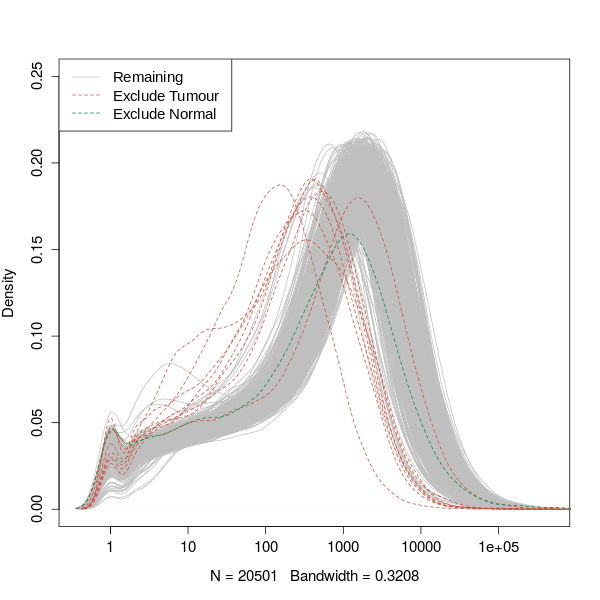
\includegraphics[width=0.55\textwidth]{fig2a.png}
        }%
        \subcaptionbox{Voom normalised}{%
           \label{fig:density:second}
           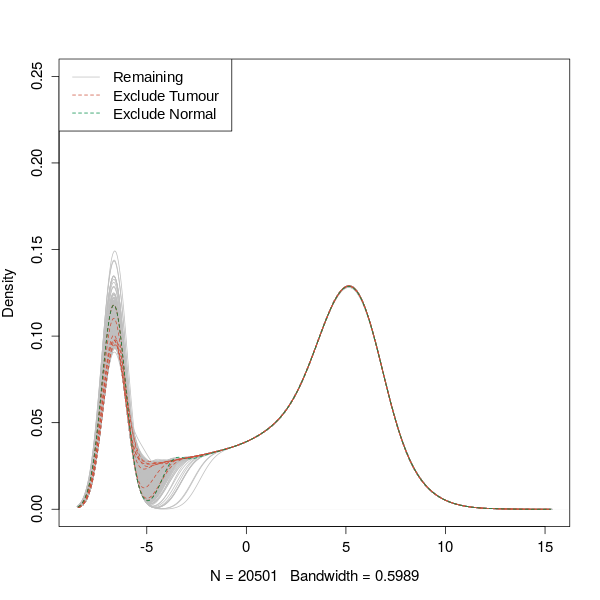
\includegraphics[width=0.55\textwidth]{fig2b.png}
        }%
%
\end{center}
\caption[Read count density]{\small \textbf{Read count density.} Sample density plots of raw counts on log-scale and voom normalised showing samples removed due to quality concerns.}
%}
\label{fig:density}
%\end{mdframed}
\end{figure*}

\begin{figure*}[!htp]
%\begin{mdframed}
%  \resizebox{\textwidth}{!}{
         \begin{center}
%
        \subcaptionbox{Mean raw counts (log-scale)}{%
            \label{fig:mean:first}
            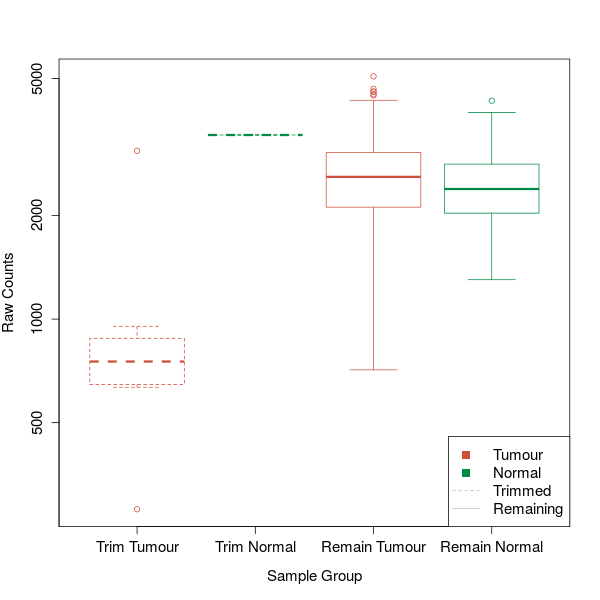
\includegraphics[width=0.55\textwidth]{fig3a.png}
        }%
        \subcaptionbox{Mean voom normalised}{%
           \label{fig:mean:second}
           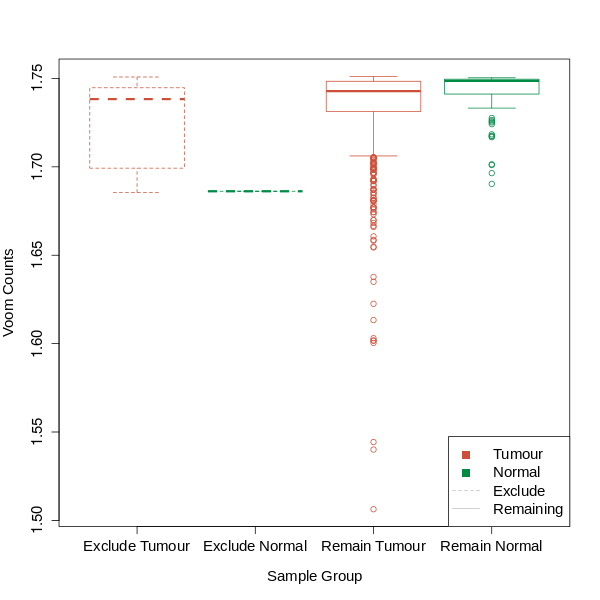
\includegraphics[width=0.55\textwidth]{fig3b.png}
        }%
%
    \end{center}
  \caption[Read count sample mean]{\small \textbf{Read count sample mean.} Boxplots of sample means for raw counts on log-scale and voom normalised show removed tumour samples with low mean read count.}
%}
\label{fig:boxplot}
%\end{mdframed}
\end{figure*}


\begin{table*}[!ht]
\caption{Excluded samples by batch and clinical characteristics.}
\label{tab:qc}
\makebox[\textwidth][c]{
\resizebox{1.25 \textwidth}{!}{
      \begin{tabular}{sc^c^c^c^c^c^c^c^c^c^c^c^c}
      \rowstyle{\bfseries}
        \multicolumn{1}{c}{\bfseries Tissue Source}		& \multicolumn{1}{sc}{\bfseries Type}   & \multicolumn{1}{sc}{\bfseries Batch} & \multicolumn{1}{sc}{\bfseries Plate} & \multicolumn{1}{sc}{\bfseries Patient} & \multicolumn{1}{sc}{\bfseries Samples} & \multicolumn{1}{c}{\bfseries p53}      & \multicolumn{1}{sc}{\bfseries Subtype}   & \multicolumn{2}{sc}{\bfseries Treatment (History)}	& \multicolumn{3}{sc}{\bfseries Clinical Subtypes (Stage)} \\
        \hline
       \rowcolor{black!10}
        A7 Christiana		& Tumour & 47	 & A227  & A0DB  &  1 of 3   & NA       & Luminal A & Mastectomy & (no)					& ER$^+$  &  Ductal   	& (2)        \\
       \rowcolor{black!5}
        A7 Christiana		& Tumour & 96	 & A220  & A13D  &  1 of 3   & Wildtype & Luminal A & Mastectomy & (no)					& ER$^+$  &  Ductal   	& (2)        \\
       \rowcolor{black!10}
        A7 Christiana		& Tumour & 96	 & A227  & A13E  &  1 of 3   & NA       & Basal     & Lumpectomy & (no) 				& ER$^-$  &  Ductal   	& (2)        \\
       \rowcolor{black!5}
        A7 Christiana		& Tumour & 142	 & A277  & A26E  &  1 of 3   & NA       & Basal     & Lumpectomy & (no) 				& ER$^+$  &  Ductal   	& (2)        \\
       \rowcolor{black!10}
        A7 Christiana		& Tumour & 47	 & A277  & A0DC  &  1 of 2   & NA       & Luminal A & Mastectomy & (yes)				& ER$^+$  &  Lobular   	& (3)        \\
       \rowcolor{black!5}
        A7 Christiana		& Tumour & 142	 & A220  & A26I  &  1 of 2   & Mutant   & Basal     & Lumpectomy & (yes) 				& ER$^-$  &  Ductal   	& (2)        \\
       \rowcolor{black!10}
        AC Intl Genom	& Tumour & 177	 & A18M  & A2QH  &  2 of 2   & Mutant   & Basal     & Radical Mastectomy & (no) 			& ER$^-$  &  Metaplastic & (2)        \\
       \rowcolor{black!5}
        AC Intl Genom	& Tumour & 177	 & A220  & A2QH  &  2 of 2   & Mutant   & Basal     & Radical Mastectomy & (no) 			& ER$^-$  &  Metaplastic & (2)        \\
       \rowcolor{black!10}
        GI ABS IUPUI		& Normal & 177	 & A16F  & A2C8  &  1 of 1   & NA       & Luminal A & \begin{tabular}{@{\hskip0pt}c@{\hskip0pt}}Radical Mastectomy \\ and Neoadjuvant \end{tabular} & (no) 	& ER$^+$  &  Ductal   	& (2)        \\
\hline
      \end{tabular}
      }}
\end{table*}

Similarly, a correlation matrix of log-transformed raw counts was used to evaluate sample quality for \gls{TCGA} stomach \gls{RNA-Seq}. A tumour sample (patient 4294) was removed due to similar quality concerns leaving a final dataset for 449 samples (from 417 patients): 414 tumour samples and 35 normal tissue samples.

\subsection{Metagenes and the Singular Value Decomposition} \label{methods:metagene}
A ``\gls{metagene}'' offers a one-dimensional summary of \gls{pathway} (expression) activation or inactivation by dimension reduction of a matrix, avoiding negatively correlated genes averaging out the signal of a mean-based centroid \citep{Huang2003}. Constructing \gls{pathway} \glspl{metagene} used gene sets for Reactome and the Gatza signatures \citep{Gatza2011, Gatza2014} as specified above (in Section~\ref{methods:gene_set}). \textcolor{red}{The singular-value decomposition ($X = U^{T} D V$) was performed on a data matrix $X$ of m genes (in the gene set) $\times$ n samples, $U$ an $m \times m$ matrix of eigenvectors of the matrix $XX^{T}$ which gives an eigenvector for each gene, $D$ is a rectangular diagonal matrix of ``singular values'' which weight the eigenvectors, and $V$ is an $n \times n$ matrix of eigenvectors of the matrix $X^{T}X$ which gives an eigenvector for each sample. The} leading eigenvector (first column of $V$) corresponding to the largest singular value was used as a \gls{metagene} for the \gls{pathway} gene set. To ensure consistent directionality of \gls{metagene} signals, the median of the gene set in each sample was calculated and correlated against the \gls{metagene} with the (arbitrary) \gls{metagene} sign adjusted as needed to conform with the majority of the gene set (i.e., positive correlation between \gls{metagene} and the median-based centroid). To ensure that genes and \glspl{pathway} were weighted equally, \glspl{metagene} were derived from a z-transformed (mean 0, standard deviation 1) dataset of \gls{gene expression} and samples were scaled (by fractional ranking) for each \gls{metagene} so that they were comparable on a $[0,1]$ scale. 

%X = an m*n matrix of data from m genes and n samples 
%U = an m*m matrix of eigenvectors of the matrix XXT which gives an eigenvector for each gene 
%D = a rectangular diagonal matrix of “singular values” which weight the eigenvectors
%V = an n*n matrix of eigenvectors of the matrix XTX which gives an eigenvector for each sample


\subsection{Candidate Triage and Integration with Screen Data} \label{methods:venn_analysis}
Candidate triage in combination with the experimental data was intended to integrate findings of the \gls{SLIPT} analysis with an ongoing experiment project \citep{Chen2014, Telford2015}. The first procedure to compare the \gls{SLIPT} gene candidates for \textit{CDH1} with an \gls{siRNA} experimental screen \citep{Telford2015} was a direct comparison of the overlapping candidates, presented in a Venn diagram and tested with the $\chi^2$ test. Since these candidates modestly overlapped at the gene level (even when excluding genes not contained in both datasets), further gene set over-representation analysis was performed for pathways specific to each detection approach and the intersection of the two.

The \gls{pathway} composition of the intersection was further verified by a permutation resampling analysis (as described in Section~\ref{methods:permutation}): the same number of genes detected by \gls{SLIPT} were sampled randomly from the universe of genes tested by both approaches. These samplings were performed over 1 million iterations and the \gls{pathway} over-representation was compared for each of the 1652 Reactome \glspl{pathway}.
%Adjusting for multiple comparisons was not needed here in a permutation analysis as the test $\chi^2$ statistics were directly used with the same degrees of freedom between expected and observed.
These over-representation scores ($\chi^2$) were compared the observed over-representation in the intersection of the \gls{SLIPT} candidates, with the proportion of resamplings with higher $\chi^2$ values used for empirical p-values of \gls{pathway} composition. The $\chi^2$ test was used as an appropriation of Fisher's exact test on a hypergeometric distribution for resampling to computationally scale \gls{pathway} over-representation tests across iterations.  Pathways for which no resamplings were occurred as high as the observed were reported as $p < 10^{-6}$. These empirical p-values were adjusted for multiple comparisons (\gls{FDR}). Intersection size was not assumed to be constant \textcolor{red}{during resampling so that it could also be used} to evaluate significance of enrichment or depletion (of \gls{siRNA} candidate among \gls{SLIPT} candidate genes).  

\section{Techniques}
Various statistical, computational, and \gls{bioinformatics} techniques were performed throughout this thesis. This Section describes these techniques and gives the parameters used unless otherwise specified. Where relevant, the R package implementation which provided the technique will be acknowledged. 

\subsection{Statistical Procedures and Tests}

As described in Sections~\ref{methods:heatmap} and~\ref{methods:metagene}, the z-transform has been used to generate z-scores in various analyses in this thesis. Each row (\textcolor{red}{$i$}) of the dataset ($x_i$) \textcolor{red}{was} transformed into a scores \textcolor{red}{vector} ($z_i$) using the mean ($\bar{x}_i$) and standard deviation ($s_i$) of the data such that:$$ z_i = \frac{\textcolor{red}{x_{i}} - \bar{x}_i}{s_i} $$
%(for each row $i$ and column $j$): $$ z_{ij} = \frac{x_{ij} - \bar{x}_i}{s_i} $$
This generates data where each row (gene) has a mean of 0 and standard deviation of 1. Where plotted as a heatmap, any data more than 3 standard deviations above or below the mean was plotted as $3$ or $-3$ respectively.

%Empirical Bayes differential \glslink{gene expression}{expression} analysis was performed using the \texttt{limma} R package \citep{limma}.
Where specified, the Fisher's exact test, $\chi^2$ test, and correlation were used to measure associations between variables, as implemented in the \texttt{stats} R package \citep{R_core}. Unless otherwise specified, Pearson correlation was used for correlation analyses ($r$) and coefficient of determination ($R^2$). Where these comparisons are discussed in more detail, Fisher's exact test and $\chi^2$ tests are supported by a table or Venn diagram, rendered with the \texttt{limma} R package \citep{limma}. In some analyses, correlation is further supported by a scatter plot and a line of best fit derived by least squares linear regression. 

The \texttt{t.test} function \citep{R_core} has also been used to implement the t-test to compare pairs of data. Where relevant, an \acrfull{ANOVA} has been performed to report significance of multivariate predictors of outcomes, or least squares linear regression performed for the adjusted coefficient of determination ($R^2$) and F-statistic p-value to evaluate the fit of the predictor variables. For some analyses these are supported by boxplot or violin plot visualisation \citep{vioplot}, rendered in R \citep{R_core}.

Multiple comparisons were accounted for with the Benjamini-Hochberg procedure to control the \gls{FDR} unless otherwise specified \citep{fdr1995}. This procedure adjusts p-values to achieve an average of the proportion of false-positives among significant tests below a threshold, $\alpha$. The more stringent Holm-Bonferroni (Holm) procedure \citep{Holm1979} was also applied in some cases to adjust for multiple comparisons and control the family-wise error rate which adjusts p-values so that the probability that any one of the tests is a false-positive (type-1 error) below a threshold, $\alpha$.

\subsection{Gene Set Over-representation Analysis} \label{methods:enrichment}
Gene set enrichment over-representation analysis was performed to test whether there was an enrichment of a gene set (e.g., a biological \gls{pathway}) among a group of input genes. Such input genes may be predicted \gls{synthetic lethal} candidates or a subset defined by clustering (in Section~\ref{methods:clustering}) or comparison with experimental candidates (in Section~\ref{methods:venn_analysis}). Initially, these tests were performed using the GeneSetDB web tool \citep{genesetdb} hosted by the University of Auckland on the Reactome \glspl{pathway} \citep{Reactome}. Since the GeneSetDB tool used an older version of Reactome (version 40), it was difficult to directly compare with the results of other analysis (in Sections~\ref{methods:venn_analysis} and~\ref{methods:permutation}) performed on version 52 (as described in  Section~\ref{methods:gene_set}). Thus an implementation of the hypergeometric test in R \citep{R_core} was used to test for over-representation against Reactome (version 52) \glspl{pathway}. Pathways containing less than 10 genes or more than 500 \citep[as performed in GeneSetDB by][]{genesetdb} were excluded before adjusting for multiple comparisons.

\subsection{Clustering} \label{methods:clustering}
The clustering analysis used unsupervised hierarchical clustering with complete linkage (distance calculated from the furthest possible pairing). For correlation matrices or multivariate normal parameters (e.g., $\Sigma$), the distance metric used was Euclidean distance. For empirical or simulated gene and \gls{pathway} \glslink{gene expression}{expression} data correlation distance was used, calculated by $distance = 1 - cor(t(x))$ where $cor$ is Pearson correlation and $t(x)$ is the transpose of the \glslink{gene expression}{expression} matrix. 

\subsection{Heatmap} \label{methods:heatmap}
Standardised z-scores of the data were used to plot heatmaps on an appropriate scale. Raw (log-scale) read counts or voom normalised counts per gene (as specified) were plotted  as normalised z-scores on a $[-3,+3]$ blue-red scale. Similarly, correlations were plotted on a $[-1,+1]$ blue-red scale. Heatmap dendrograms were generated using the linkage method and distance specified for the clustering performed in Section~\ref{methods:clustering}. The \texttt{gplots} R package \citep{gplots} was used to generate many of the heatmaps throughout this thesis, along with a customised heatmap function (released as \texttt{heatmap.2x}, detailed in Table~\ref{tab:computers_r_packages_dev} and Section~\ref{methods:r_packages_vis}). Where clearly specified, data have been split into subsets with clustering performed separately on each subset with these plotted alongside each other.

\subsection{Modelling and Simulations} \label{methods:simulation}
Statistical modelling and simulations were used to test various \gls{synthetic lethal} detection procedures on simulated data. This involved constructing a statistical model of how \glspl{synthetic lethal} would appear in (continuous normally distributed) \gls{gene expression} data. Where presented (in Section~\ref{methods:SL_Model}), the assumptions of the model are stated clearly. The model allows sampling from a multivariate normal distribution (using the \texttt{mvtnorm} R package \citep{Genz2009, mvtnorm}) to generate simulated data with known underlying \gls{synthetic lethal} partners (detailed in Section~\ref{methods:simulating_SL}). I can test whether statistical procedures, including those developed in this thesis (presented in Section~\ref{methods:SLIPT}), are capable of detecting \gls{synthetic lethal} partners within the simulated data. This multivariate normal simulation procedure also enables the inclusion of correlation structure which is either given as correlated blocks of genes or derived from \glslink{graph}{pathway} structures (as detailed in Section~\ref{methods:graphsim}).

When this multivariate normal distribution is sampled once and the procedure to add known \gls{synthetic lethal} partners is performed, it generates a simulated dataset. Performing this simulation procedure and testing with a \gls{synthetic lethal} detection procedure iteratively, these simulations can be used to assess the statistical performance of the detection procedure. The number of iterations (\texttt{Reps}) will be given for each simulation result. Typically, these are performed 1000 or 10,000 times depending on \textcolor{red}{the} computational feasibility of doing so on larger datasets. 

Several measures of statistical performance were used to assess the simulations. The following measures used the final classification of the detection procedure, statistical significance for $\chi^2$, significance and directional criteria met for \gls{SLIPT} (in Section~\ref{methods:SLIPT}), and an arbitrary threshold: $r < -0.2$ and $r >+0.2$ for  negative correlation and correlation respectively. \textcolor{red}{The significance thresholds (of FDR adjusted $p<0.05$) were applied for SLIPT and $\chi^2$ as used throughout thesis. The thresholds for correlation were used to classify a meaningful number of genes (several hundred) to test the methodology. This threshold does not affect the statistical performance from which the main conclusions are drawn}. Sensitivity (or ``true positive rate'') was measured as the proportion of known \gls{synthetic lethal} partners predicted to be \gls{synthetic lethal}. Specificity (or ``true negative rate'') was measured as the proportion of known non-synthetic lethal partners predicted not to be \gls{synthetic lethal}. The ``false positive rate'' was measured here as the proportion of known non-synthetic lethal partners out of all putative partners predicted by the detection procedure. Statistical ``accuracy'' is the proportion of true predictions for a detection procedure, which is both the correctly predicted known \gls{synthetic lethal} partners and correctly negative known non-synthetic lethal partners.

\subsubsection{Receiver Operating Characteristic Curves} \label{methods:ROC} \glsreset{ROC} \glsreset{AUROC}
A more general procedure to measure the statistical performance of a simulation is the \gls{ROC} curve which does not assume a threshold for classification of \glspl{synthetic lethal} but demonstrates the achievable range of sensitivity and specificity for a model \citep{Zweig1993, Fawcett2006, Akobeng2007}. These curves (implemented with the \texttt{ROCR} R package \citep{ROCR}) plot the true positive rate (sensitivity) against the false positive rate ($1-$specificity) as the prediction threshold is varied. An ideal detection method will have a true positive rate of 1 and a false positive rate of 0, hence the Area Under the \gls{ROC} curve (AUC or \gls{AUROC}) is a measure of statistical performance for a detection procedure accounting for this trade-off. \gls{AUROC} values typically range from 0.5 (the value expected by random chance) to 1 for an optimal detection method, however it is possible for an \gls{AUROC} below 0.5 for a poor detection method that performs worse than random chance. In cancer biology, it has been suggested that an \gls{AUROC} of approximately $0.8$ is a predictive biomarker suitable for publication \citep{Hajian-Tilaki2013} but predictors with lower \gls{AUROC} values may still be informative depending on the context. In this thesis, the \gls{AUROC} values varied widely across simulation parameters and were primarily used for comparisons across these parameters, although they can also be used to refine thresholds for optimal classification. 

\subsection{Resampling Analysis} \label{methods:permutation}
Resampling analyses (e.g., ``permutation'' analysis) are used to statistically test the significance of an observation without assuming the underlying distribution of expected test statistics \citep{Collingridge2013}. Instead these are derived from randomly shuffling test statistics or randomly sampling predicted candidates. For the purposes of this thesis, this involved randomly sampling genes from those tested to be analysed as putative \gls{synthetic lethal} candidates. This was performed both for testing the significance of \gls{pathway} composition in the intersection with experimental gene candidates (Section~\ref{methods:venn_analysis}) and for assessing the significance of \glslink{graph}{pathway} structure among \gls{synthetic lethal} candidates (Section~\ref{methods:network_permutation}).

These were analysed to compare the observed \gls{synthetic lethal} genes against values derived from randomly sampling the same number of genes as were observed to be \gls{synthetic lethal} from among the genes tested. Sampling iteratively across many resampling procedures, these resampling-based values form a null distribution that could be expected if the null hypothesis were true. Thus the proportion of resampling-based values across these iterations that are greater than or equal to that observed, forms an empirically derived p-value to test significance.

Resampling was performed for comparison (in Section~\ref{methods:venn_analysis}) with fixed experimental screen candidates \citep{Telford2015} both resampling the number of genes overlapping with the screen candidates and test statistics for \gls{pathway} enrichment. Resampling analysis was also applied to \glspl{shortest path} and network metrics (in Section~\ref{methods:network_permutation}) to test significance of directional relationships between \gls{synthetic lethal} candidate genes within \glslink{graph}{pathway} structures.

The number of iterations determines the accuracy of these p-values. For \gls{pathway} composition (in Section~\ref{methods:venn_analysis}), a million iterations were performed using high performance computing (as detailed in Section~\ref{methods:HPC}) to provide sufficient accuracy after adjusting for multiple comparisons across \glspl{pathway}. For the purposes of network analysis (in Section~\ref{methods:network_permutation}), a thousand iterations were sufficient to reject the null hypothesis for the majority of \glspl{pathway} tested before adjusting for multiple comparisons, and thus further iterations were not performed.

\section{Pathway Structure Methods}

\subsection{Network and Graph Analysis}

Networks are important in considering the structure of relationships in molecular biology, including gene regulation, kinase cellular signalling, and metabolic \glspl{pathway} \citep{Barabasi2004}. Network theory is an interdisciplinary field which combines the approaches of computer science with the metrics and fundamental principles of graph theory, an area of pure mathematics dealing with relationships between sets of discrete elements. The vast amounts of molecular and cellular data from high-throughput technologies have enabled the application of network-based and \glspl{genome}-wide \gls{bioinformatics} analysis to examine the complexity of a cell at the molecular level and understand aberrations in cancer. This thesis uses various metrics and analysis procedures developed in Graph and Network theory to analyse \glslink{graph}{graph} structure of biological \glspl{pathway}. Where feasible, these have been implemented using the \texttt{igraph} R package with such procedures described below \citep{igraph}. Custom R functions were used to perform more complex analysis and visualisation of iGraph data (as described in Section~\ref{methods:igraph_extensions}).

Graph theory is a branch of pure mathematics which deals with the properties of sets of discrete objects (referred to as a `node' or `vertex`) with some pairs are joined (by a `link' or an `edge`). While a seemingly reductionist abstraction to mathematically study relationships, graph theory has applications in a wide range of fields, including the life sciences. Network theory is the sub-discipline of graph theory that deals with networks, which has become popular due to the vast potential for applications of networks \citep{vanSteen2010}. 

Applications vary depending on the situation modelled, particularly in how the \glspl{edge} between \glspl{vertex} are defined, whether they are directed or weighted, and whether multiple redundant \glspl{edge} between a pair of \glspl{vertex} (referred to as `parallel \glspl{edge}`) or \glspl{edge} connecting a \glslink{vertex}{vertex} to itself (referred to as `loops`) are permitted in the model. Networks are defined such that the \glspl{edge} represent a relationship between the \glspl{vertex} and may be directed, weighted, or contain parallel \glspl{edge} or loops depending on the application \citep{vanSteen2010}. Unless otherwise stated, \glslink{graph}{graph} structures and networks in this thesis will be unweighted and have no parallel \glspl{edge} or loops. Where a directional relationship is known or modelled, it will be represented with a directed \glslink{edge}{edge} in a directed graph.

\subsection{Sourcing Graph Structure Data} \label{methods:graph_data}
Pathway Commons interaction data was sourced using the \gls{BioPAX} with the paxtools-4.3.0 Java application on October 6\textsuperscript{th} 2015 \citep{PathwayCommons, paxtools}. This utility was used to import`sif' format interaction data into R \citep{R_core} and extract the human Reactome (version 52) dataset of interactions was imported \citep{Reactome}, matching those used for \gls{pathway} enrichment analysis. These interactions were used to construct an adjacency matrix \textcolor{red}{($A_{ij}$ for row $i$ and column $j$)} for the Reactome network and subnetworks corresponding to each relevant biological \gls{pathway}. 
\textcolor{red}{
\[
A_{ij} = 
\begin{dcases*}
   1                         & if genes $i$ and $j$ are adjacent \\
   0                         & otherwise
\end{dcases*}
\]
}
\subsection{Constructing Pathway Subgraphs} \label{methods:subgraphs}
Subgraphs for each relevant \gls{pathway} were constructed by matching the \glslink{vertex}{nodes} in the complete Reactome network to the \gls{pathway} gene sets (as derived in Section~\ref{methods:gene_set}). A subgraph with adjacent \glslink{vertex}{nodes} was constructed by adding \glslink{vertex}{nodes} which have an \glslink{edge}{edge} with a gene in the \gls{pathway} gene set. The \glspl{pathway} these adjacent \glslink{vertex}{nodes} belong to were added to form a ``meta-\gls{pathway}'' to account for the possibility for \glslink{vertex}{nodes} within the \gls{pathway} being linked by the surrounding \glslink{graph}{graph} structure.

\subsection{Network Analysis Metrics} \label{methods:network_metrics}
The existing network analysis measures applied in this thesis (as described below) used an implementation in the \texttt{igraph} R package to compute vertex degree, shortest paths, and centrality \citep{igraph}. Additionally, custom features were developed for analysis of iGraph objects in R and released as \texttt{igraph.extensions} (as described in Section~\ref{methods:igraph_extensions}).

Vertex degree is the number of \glspl{edge} a \glslink{vertex}{node} has and is a fundamental measure of the importance and connectivity of a network \citep{vanSteen2010}. More connected \glslink{vertex}{nodes}, such as network hubs, will have a higher \glslink{vertex}{vertex} degree relative to other \glslink{vertex}{nodes}. For the purposes of this thesis, \glslink{vertex}{vertex} degree ignored \glslink{edge}{edge} direction with loops (edges with itself) and double \glspl{edge} to the same \glslink{vertex}{node} excluded.

A fundamental concept in network analysis is a ``\gls{shortest path}'', that is the shortest route via \glspl{edge} between any two particular \glslink{vertex}{nodes} in a network. These are computed by Dijstra's algorithm \citep{Dijkstra1959} in the \texttt{igraph} R package \citep{igraph}. Where applicable paths will only use directed \glspl{edge} in a particular direction. Shortests paths are a useful measure of how close \glslink{vertex}{nodes} are in a network. This is used to compute \gls{information centrality}, and for further analysis of \glslink{graph}{pathway} structure (as described in Section~\ref{methods:pathway_str}).

Network \gls{centrality} is an alternative measure of the importance or influence of a \glslink{vertex}{node} to the \glslink{graph}{graph} structure \citep{Borgatti2005}. Various strategies are used to derive centrality,  typically based on how connected the \glslink{vertex}{node} is or the impact of \glslink{vertex}{node} removal on the connectivity of the network. One of the most notable is the ``\glslink{PageRank centrality}{PageRank}'' algorithm, a refinement of eigenvector \gls{centrality} based on the eigenvectors of the adjacency matrix \citep{Brin1998}. This is implemented in the \texttt{igraph} R package \citep{igraph}.

Another network \gls{centrality} measure that has been previously applied to biological protein interaction networks \citep{Kranthi2013} is the ``\gls{information centrality}''. The \gls{information centrality} of a \glslink{vertex}{node} is the relative impact on efficiency (transmission of information via \glspl{shortest path}) of the network when the \glslink{vertex}{node} is removed. \textcolor{red}{The} \gls{centrality} ($C$) \citep{Kranthi2013} for \glslink{vertex}{node} $n$ in \textcolor{red}{a} graph $G$ \textcolor{red}{(containing $N$ nodes)} is defined as: $$C_n = \frac{E(G)-E(G')}{E(G)}$$ where $G'$ is the subgraph with the \glslink{vertex}{node} removed and $E$ is the efficiency \citep{Latora2001}, derived from \glspl{shortest path} ($d_{ij}$ between \glslink{vertex}{nodes} $i$ and $j$). $$E(G) = \frac{2}{N(N-1} \sum_{i<j \in G}^{} \frac{1}{d_{ij}}$$ The efficiency of a network can be derived from \glspl{shortest path} \textcolor{red}{using the} \texttt{igraph} R package and the network \gls{centrality} computation for each \glslink{vertex}{node} has been released as an R package (\texttt{info.centrality}) and included in the \texttt{igraph.extensions} package.

%%move graph structure methods to Chapter 2? (if Chapter 3 renamed)

\section{Implementation}
%\subsection{Computational Tools and Enabling Biological Research (remove/state assumptions only)}
%\subsubsection{Computational Tools for Biological Research}
%In addition to hosting data repositories on the web, tools developed with computational expertise have had wider benefit in  genetics research. One of the main impacts of a techniques developed from computer science is the alignment of reads, to either assemble a \glspl{genome} \textit{de novo} from its reads or map reads to a pre-existing reference \glspl{genome}. Mapping reads is commonplace to call variants between samples, this is useful for studies of human disease interested in risks of these variants or wider application such as comparing populations or species in an evolution phylogeny. Mapping reads has further utility in functional genetics to identify which regions or a \glspl{genome} are expressed or have \acrshort{DNA} methylation. Similarly, mapping is used to map \gls{RNA-Seq} or Bisulfite-Seq reads to measure \gls{gene expression} or \acrshort{DNA} methylation across the \glspl{genome} in a cohort or sample. While mapping is not performed in this thesis, it has performed an important role in the adoption of \glspl{genomic} in genetics research.



\subsection{Computational Resources and Linux Utilities}

Several computers were used to process and store data during this thesis (as summarised in Appendix Table~\ref{tab:computers}), running different versions of Linux operating systems, including a personal laptop computer, laboratory desktop machine, departmental server, and the New Zealand eScience Infrastructure Intel Pan high-performance computing cluster (a supercomputer based at the University of Auckland). Each of these systems support a 64-bit architecture. Current workflows on local machines use Elementary OS (based on the Ubuntu versions given in Appendix Table~\ref{tab:computers}) and the ZSH shell. However, Ubuntu OS and the Bash were used at the inception of this project and Bash continues to be used for running scripts. Various Linux applications and command-line utilities were used on these machines (shown in Appendix Table~\ref{tab:computers_linux}). As such, the workflows developed in this project should be backwards-compatible with Ubuntu Linux (and other derivatives). The majority of novel methodology and implementations were performed in R which is a cross-platform language, packages developed in R will be available for users of Linux, Mac, and Windows machines.  


\FloatBarrier

\subsection{R Language and Packages}


The R programming language has been used for the majority of this thesis. Current R installations across the machines used are given in Table~\ref{tab:computers_r}. Local machines currently run the latest version of the R (at the time of writing) and remote machines run the versions and modules as managed by the system administrator.

Various scripts and packages in this thesis were developed or run in previous versions of RStudio and R but these run without error in the current version of R (and the older versions on remote machines). The R packages which were used throughout this thesis (as detailed in Table~\ref{tab:computers_r_packages} with versions specified) were installed from the \acrfull{CRAN} \citep{CRAN}, Bioconductor \citep[][version 3.4; BiocInstaller 1.24.0]{Gentleman2004}, or GitHub (\url{https://github.com/}). These packages were not updated when they would change the functionality of scripts or functions in packages\textcolor{red}{. In particular,} imported data from annotation packages (used to define gene sets) have been saved as local files to continue using stable versions of these \gls{pathway} data (across machines).

This is a summary of the key packages which (in addition to their dependencies) have been used throughout this project. Where a package implementation has been central to the methods applied, they are described in more detail in the relevant Section. A full table of packages used in this thesis can be found in Appendix Table~\ref{tab:computers_r_packages_full}. The R packages developed during this thesis are given in Table~\ref{tab:computers_r_packages_dev} with the relevant Sections describing their implementation and use where appropriate, in addition to further details on these functions in Section~\ref{methods:r_packages}. 

\begin{table}[!ht]
\centering
\caption{R installations used during thesis}
\label{tab:computers_r}
\resizebox{\textwidth}{!}{
\begin{tabular}{|ll|l|l|l|l|}
%\cline{3-6}
\multicolumn{1}{l}{\cellcolor{white}}   & \multicolumn{1}{l}{}              & \multicolumn{1}{l}{\bfseries Viao Laptop}                           & \multicolumn{1}{l}{\bfseries Lab Machine}                         & \multicolumn{1}{l}{\bfseries Biochem Server}                           & \multicolumn{1}{l}{\bfseries NeSI Pan Cluster}           \\
\cline{2-6}
\rowcolor{black!10}
\multicolumn{1}{l}{\cellcolor{white}}   & \multicolumn{1}{|l|}{OS}          & \begin{tabular}[c]{@{}l@{}}Elementary OS\\ Freya 0.3.2\end{tabular} & \begin{tabular}[c]{@{}l@{}}Elementary OS\\ Loki 0.4\end{tabular}  & \begin{tabular}[c]{@{}l@{}}Red Hat Enterprise\\ Maipo 7.2\end{tabular} & \begin{tabular}[c]{@{}l@{}}Cent OS\\ Final 6.4\end{tabular} \\
\hline
\rowcolor{black!5}
\cellcolor{white} Programming           & \multicolumn{1}{|l|}{R}           & 3.3.2                                                               & 3.3.2                                                             & 3.3.1                                                                  & 3.3.0-intel (module)                          \\
\hline

\rowcolor{black!10}
\cellcolor{white} Development           & \multicolumn{1}{|l|}{RStudio}     & 1.0.136                                                             & 1.0.136                                                           & 1.0.136 (server)                                                       &                                                \\
\hline
\end{tabular}
}
\end{table}

%\resizebox{\textwidth}{!}{
\setlength{\LTleft}{-20cm plus -1fill}
\setlength{\LTright}{\LTleft}

\begin{longtable}{llll}
\caption{R Packages used during thesis}
\label{tab:computers_r_packages}
%\\ hline
\\
\multicolumn{1}{l}{\bfseries Package}      & \multicolumn{1}{l}{\bfseries Version Used} & \multicolumn{1}{l}{\bfseries Built} & \multicolumn{1}{l}{\bfseries Repository}      \\
\hline  \rowcolor{black!10}
colorspace   & 1.3-2          & 3.3.1 & \gls{CRAN}            \\
%\hline  
\rowcolor{black!5}
curl         & 2.3            & 3.3.1 & \gls{CRAN}            \\
%\hline  
\rowcolor{black!10}
data.table   & 1.9.6          & 3.3.1 & \gls{CRAN}            \\
%\hline  
\rowcolor{black!5}
dendextend   & 1.4.0          & 3.3.2 & \gls{CRAN}            \\
%\hline  
\rowcolor{black!10}
DBI          & 0.5-1          & 3.3.1 & \gls{CRAN}            \\
%\hline  
\rowcolor{black!5}
devtools     & 1.12.0         & 3.3.1 & \gls{CRAN}            \\
%\hline  
\rowcolor{black!10}
dplyr        & 0.5.0          & 3.3.1 & \gls{CRAN}            \\
%\hline  
\rowcolor{black!5}
ggplot2      & 2.2.1          & 3.3.1 & \gls{CRAN}            \\
%\hline  
\rowcolor{black!10}
git2r        & 0.18.0         & 3.3.1 & \gls{CRAN}            \\
%\hline  
\rowcolor{black!5}
gplots       & 3.0.1          & 3.3.1 & \gls{CRAN}            \\
%\hline  
\rowcolor{black!10}
gtools       & 3.5.0          & 3.3.1 & \gls{CRAN}            \\
%\hline  
\rowcolor{black!5}
igraph       & 1.0.1          & 3.3.1 & \gls{CRAN}            \\
%\hline  
\rowcolor{black!10}
matrixcalc   & 1.0-3          & 3.3.1 & \gls{CRAN}            \\
%\hline  
\rowcolor{black!5}
mclust       & 5.2.2          & 3.3.1 & \gls{CRAN}            \\
%\hline  
\rowcolor{black!10}
mvtnorm      & 1.0-6          & 3.3.1 & \gls{CRAN}            \\
%\hline  
\rowcolor{black!5}
org.Hs.eg.db & 3.1.2          & 3.1.2 & Bioconductor    \\
%\hline  
\rowcolor{black!10}
openssl      & 0.9.6          & 3.3.1 & \gls{CRAN}            \\
%\hline  
\rowcolor{black!5}
plyr         & 1.8.4          & 3.3.1 & \gls{CRAN}            \\
%\hline  
\rowcolor{black!10}
purrr        & 0.2.2          & 3.3.1 & \gls{CRAN}            \\
%\hline  
\rowcolor{black!5}
reactome.db  & 1.52.1         & 3.2.1 & Bioconductor    \\
%\hline  
\rowcolor{black!10}
RColorBrewer & 1.1-2          & 3.3.1 & \gls{CRAN}            \\
%\hline  
\rowcolor{black!5}
Rcpp         & 0.12.9         & 3.3.1 & \gls{CRAN}            \\
%\hline  
\rowcolor{black!10}
ROCR         & 1.0-7          & 3.3.1 & \gls{CRAN}            \\
%\hline  
\rowcolor{black!5}
roxygen2     & 6.0.1          & 3.3.2 & \gls{CRAN}            \\
%\hline  
\rowcolor{black!10}
shiny        & 1.0.0          & 3.3.1 & \gls{CRAN}            \\
%\hline  
\rowcolor{black!5}
snow         & 0.4-2          & 3.3.1 & \gls{CRAN}            \\
%\hline  
\rowcolor{black!10}
testthat     & 1.0.2          & 3.3.2 & \gls{CRAN}            \\
%\hline  
\rowcolor{black!5}
tidyr        & 0.6.1          & 3.3.2 & \gls{CRAN}            \\
%\hline  
\rowcolor{black!10}
tidyverse    & 1.1.1          & 3.3.2 & GitHub (hadley) \\
%\hline  
\rowcolor{black!5}
sm           & 2.2-5.4        & 3.3.1 & \gls{CRAN}            \\
%\hline  
\rowcolor{black!10}
Unicode      & 9.0.0-1        & 3.3.2 & \gls{CRAN}            \\
%\hline  
\rowcolor{black!5}
vioplot      & 0.2            & 3.3.1 & \gls{CRAN}            \\
%\hline  
\rowcolor{black!10}
viridis      & 0.3.4          & 3.3.2 & \gls{CRAN}            \\
%\hline  
\rowcolor{black!5}
xml2         & 1.1.1          & 3.3.2 & \gls{CRAN}            \\
%\hline  
\rowcolor{black!10}
xtable       & 1.8-2          & 3.3.1 & \gls{CRAN}            \\
%\hline  
\rowcolor{black!5}
zoo          & 1.7-14         & 3.3.1 & \gls{CRAN}            \\
%\hline  
\rowcolor{black!10}
graphics     & 3.3.2          & 3.3.2 & base            \\
%\hline  
\rowcolor{black!5}
grDevices    & 3.3.2          & 3.3.2 & base            \\
%\hline  
\rowcolor{black!10}
cluster      & 2.0.5          & 3.3.1 & base            \\
%\hline  
\rowcolor{black!5}
Matrix       & 1.2-8          & 3.3.1 & base            \\
%\hline  
\rowcolor{black!10}
stats        & 3.3.2          & 3.3.2 & base            \\
\hline
\end{longtable}

\begin{table}[!ht]
\centering
\caption{R packages developed during thesis}
\label{tab:computers_r_packages_dev}
\makebox[\textwidth][c]{
\resizebox{1.25 \textwidth}{!}{
\begin{tabular}{|l|llc|}
%\cline{2-4}
\multicolumn{1}{l}{}           & \multicolumn{1}{l}{\bfseries Package Name} & \multicolumn{1}{l}{\bfseries Description                                                   and GitHub Repository}                                                                   & \multicolumn{1}{c}{\bfseries Section} \\
\cline{2-4}  \rowcolor{black!10}
\multicolumn{1}{l|}{\cellcolor{white}}           & \multicolumn{1}{l}{\texttt{slipt}}        & \begin{tabular}[c]{@{}l@{}}Synthetic lethal detection by \gls{SLIPT} (to accompany publication)  \\ \url{https://github.com/TomKellyGenetics/slipt}                         \end{tabular} & \ref{methods:SLIPT}  \\
\hline
\rowcolor{black!5} \cellcolor{white}
visualisation                  & \texttt{vioplotx}                          & \begin{tabular}[c]{@{}l@{}}Customised violin plots (based on \texttt{vioplot})             \\ \url{https://github.com/TomKellyGenetics/vioplotx}                      \end{tabular} &                              \\
%\cline{2-4}
\rowcolor{black!10} \cellcolor{white}
                               & \texttt{heatmap.2x}                      & \begin{tabular}[c]{@{}l@{}}Customised heatmaps (based on \texttt{gplots})                  \\ \url{https://github.com/TomKellyGenetics/heatmap.2x}                    \end{tabular} & \ref{methods:heatmap} \\
\hline
\rowcolor{black!5} \cellcolor{white}
\texttt{igraph.extensions}     & \texttt{igraph.extensions}               & \begin{tabular}[c]{@{}l@{}}Meta-package to install the follow iGraph functions             \\ \url{https://github.com/TomKellyGenetics/igraph.extensions}             \end{tabular} & \ref{methods:igraph_extensions}    \\
%\cline{2-4}

\rowcolor{black!10} \cellcolor{white}
                               & \texttt{plot.igraph}                     & \begin{tabular}[c]{@{}l@{}}Custom plotting of directed \glspl{graph}                              \\ \url{https://github.com/TomKellyGenetics/plot.igraph}                   \end{tabular} & \ref{methods:network_metrics}      \\
%\cline{2-4}
\rowcolor{black!5} \cellcolor{white}
                               & \texttt{info.centrality}                 & \begin{tabular}[c]{@{}l@{}}Computing \gls{information centrality} from network efficiency        \\ \url{https://github.com/TomKellyGenetics/info.centrality}               \end{tabular} & \ref{methods:graphsim}\\
%\cline{2-4}

\rowcolor{black!10} \cellcolor{white}
                               & \texttt{pathway.structure.permutation}   & \begin{tabular}[c]{@{}l@{}}Testing \glslink{graph}{pathway} structure with resampling analysis              \\ \url{https://github.com/TomKellyGenetics/} \\ \textcolor{blue!80!white}{\texttt{pathway.structure.permutation}} \end{tabular} & \ref{methods:network_permutation}  \\
%\cline{2-4}
\rowcolor{black!5} \cellcolor{white}
                               & \texttt{graphsim}                        & \begin{tabular}[c]{@{}l@{}}Generating simulated \glslink{gene expression}{expression} from \glslink{graph}{graph} structures           \\ \url{https://github.com/TomKellyGenetics/graphsim}                      \end{tabular} & \ref{methods:graphsim}\\
\hline 
\end{tabular} 
}}
\end{table}

%\FloatBarrier

\subsection{High Performance and Parallel Computing} \label{methods:HPC}
\glsreset{HPC}
\glsreset{NeSI}
\glsreset{Slurm}

Another enabling technology for \gls{bioinformatics} is parallel computing, performing independent operations using separate \gls{CPU} cores: this ``multithreading'' is widely used to \textcolor{red}{de}crease the time to compute results. \Gls{bioinformatics} is particularly amenable to this since performing multiple iterations of a simulation or testing separate genes is often ``embarrassingly parallel'', as \glspl{CPU} completely independent of each other. %As such, parallel computing is offered by many high-performance ``supercomputers'', including national research infrastructure.

\Gls{NeSI} is a \gls{HPC} organisation providing the Intel Pan cluster or ``supercomputer'' at the University of Auckland \citep{NeSI}. The cluster was used throughout this thesis project to optimise and perform computations which would have otherwise been infeasible. High performance computing on the Pan cluster was used extensively in this project including for resampling analysis (in Sections~\ref{methods:permutation} and~\ref{methods:network_permutation}), calculating \gls{information centrality} (in Section~\ref{methods:network_metrics}), and in simulations (in Sections~\ref{methods:simulation},~\ref{methods:simulation_SL_expression}, and~\ref{methods:graphsim})

Scripts and data were transferred between the Pan cluster and University of Otago computing resources by \texttt{rsync} or the Globus file transfer service \citep{Globus}. R scripts \citep{R_core} were run in parallel with the ``simple network of workstations'' \texttt{snow} R package \citet{snow}. This utilised the ``message passing interface'' \citep{Rmpi} when it was feasible with memory requirements to run in parallel across multiple compute \glslink{vertex}{nodes}, otherwise \gls{SOCKS} was used to access multiple cores within an instance of R and pass input data to them. R jobs were submitted to queue for available resources and run on the Pan cluster via the \gls{Slurm} workload manager \citep{slurm}.  \gls{Slurm} array job submission and independent running of different parameters (with arguments passed to R from the shell) were used to run memory-intensive job or scripts across many parameters simultaneously. In some cases, this submission was automated across a range of parameters with Bash scripts.

%\subsection*{Comparison Subsetting}
%\subsubsection*{Comparison to Experimental Screen}
% Comparison to screen validation data utilised primary screen data from a cell line experiment by Telford \textit{et al.} \citet{Telford2015} using the \gls{synthetic lethal} selection criteria defined by the authors based on gene knockout viability in isogenic MCF10A breast cell lines. A direct comparison was implemented using Venn diagrams from the \texttt{limma} package in R \citep{limma}. This comparison used a `universe' of all 16,298 genes tested by both methods, which had sufficient non-zero variation to define 3-quantiles in the \gls{TCGA} \glslink{gene expression}{expression} dataset \citep{TCGA2012} and had \gls{siRNA} targets in the primary screen \citep{Telford2015}, excluding any genes not tested by one of these approaches. A $\chi^2$ test was performed on this reduced universe to test for association between each \gls{synthetic lethal} identification approach.

%\subsubsection*{Gene Set Analysis}
%Gene set over-represent\-ation was tested for genes within each sector of the Venn diagram to compare pathways specific to each approach to those identified by both. This over-represent\-ation analysis was performed using the hypergeometric test implemented in R as described below \citep{HyperGeo, R_core}. Further analysis of the intersection of these approaches was performed using the resampling procedure as described below.

%\subsection*{Pathway Analysis}
%\subsubsection*{Pathway Over-representation Analysis}
%Pathway over-represent\-ation analysis was performed using the \texttt{phyper} function of the R stats package unless specified otherwise \citep{HyperGeo, R_core}. This performs a hypergeometric test for over-represent\-ation of members of a pathway in a given group of genes as suggested by \citet{Rivals2007}. 1652 pathways were defined using the Reactome database \citep{Reactome} (version 52). Pathway over-represent\-ation used a `universe' of genes tested by both approaches for the intersection, as in the Venn analysis above, and otherwise used all of the genes tested by the respective approach. 1030 Reactome pathways were used with a size filtering criteria of containing at least 10 genes and no more than 500 genes, as recommended \citet{genesetdb}.

%\subsubsection*{Pathway Resampling Analysis}
%Resamping was performed to test whether over-represented pathways were to be expected between the two methods by chance. The number of predicted genes from \gls{SLIPT} (4,629) was sampled randomly without replacement from the gene `universe' as defined by the Venn diagram in Figure~\ref{fig:Venn_allgenes}, and as described above.  This sample was compared to the 2203 experimental \gls{synthetic lethal} candidates from screen data \citep{Telford2015} that were tested by \gls{SLIPT} to resample the intersection between computationally and experimentally identified \gls{synthetic lethal} candidates. For both the sample from universe gene set and the intersection with experimental screen candidates, a $\chi^2$ test was performed for association with each of the Reactome pathways for a computationally feasible measure of pathway over-represent\-ation.

%This procedure was repeated in parallel over 1 million replicates using the \texttt{snow} and \texttt{Rmpi} R packages \citep{snow, Rmpi} to generate a null distribution of $\chi^2$ values for each Reactome pathway. An estimate of significance for each pathway was generated as a empirical p-value from the proportion of 1 million $\chi^2$ expected values from random samples that exceeded the $\chi^2$ value observed performing the same over-represent\-ation procedure on the predicted \gls{synthetic lethal} candidates for \textit{CDH1} from \gls{SLIPT}. Note that the above procedure does not assume a fixed intersection size and the expected distribution also can be compared to the observed number of intersection genes in a similar manner. 

%\subsubsection*{Pathway Metagene Analysis}
%insert text

%\subsection*{Heatmap Procedure}
%\subsubsection*{Parameters}
%Heatmaps were generated in R using modifications to the \texttt{heatmap.2} from the \texttt{gplots} package \citep{gplots} (with annotation modifications documented in the \texttt{heatmap.2x} R package on GitHub: \url{https://github.com/TomKellyGenetics/heatmap.2x}.

%\subsubsection*{Correlation matrix}
%Pairwise Pearson correlation between samples (log-scale) were plotted with Euclidean distance and complete linkage on a $[-1,1]$ blue-red scale.
%\subsubsection*{Expression (gene) matrix}
%Raw (log-scale) read counts or voom normalised counts per gene (as specified) were plotted with correlation (Pearson) distance and complete linkage as normalised z-scores on a $[-3,+3]$ blue-red scale.
%\subsubsection*{Expression (metagene) matrix}
%raw (log-scale) read counts or voom normalised counts per gene (as specified) were as normalised z-scores on a $[-3,+3]$ scale and used for generating pathway \glspl{metagene} which were plotted with Correlation (Pearson) distance and complete linkage on a ranked $[0,1]$ blue-red scale.
%\subsubsection*{Annotation}
%\gls{TCGA} clinical and \gls{mutation} data is plotted as colour bars above heatmaps on a continuous red-blue spectrum, or as discrete colours as described in legends or figure captions. All clinical and molecular data comes from \gls{TCGA} \citep{TCGA2012} or ICGC \citep{Zhang2011} sources apart from \gls{PAM50} \glspl{intrinsic subtype} which was %<downloaded from the University of California Santa Cruz website from \gls{microarray} data in 2012> OR 
%calculated using the \gls{PAM50} methodology as described by \citet{Parker2009} from \gls{RSEM} normalised \gls{RNA-Seq} data using centroids provided by J.S. Parker (personal communication). %in 2015
%Row annotation bars contain similar colours, which correspond to genes in \glslink{gene expression}{expression} data, factors including genes in pathway datasets, experimental, and computational results again on a red-blue colour spectrum or discrete colours as described accompanying each figure. 

%\subsection*{Implementation}
%All analyses were performed via R \citep{R_core} and custom shell scripts using local and national computing infrastructure. Novel analysis approaches for \glspl{synthetic lethal} are available in the \texttt{slipt} R package on GitHub (\url{http://github.com/TomKellyGenetics/slipt}) while other analyses used various Bioconductor packages to annotate and process genetic data \citep{Gentleman2004} (\url{http://bioconductor.org}).
